\chapter{System Design and Architecure}
\section{USE CASE DIAGRAM}
\begin{figure}[H]
    \centering
    \vspace{1.5cm}
    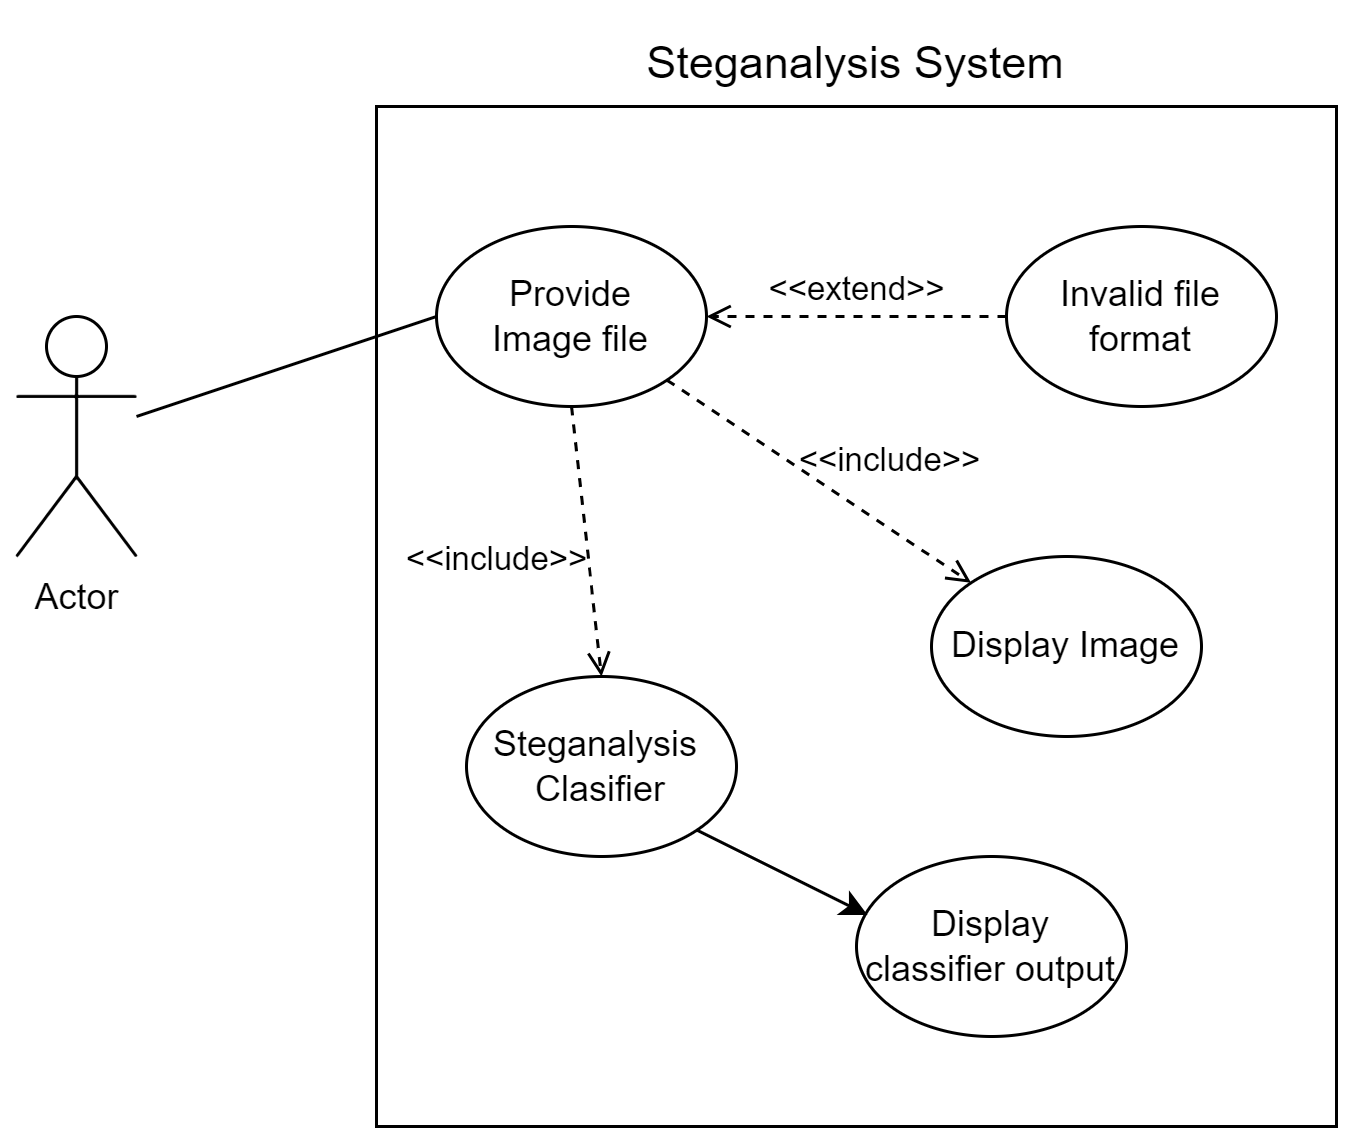
\includegraphics[width=120mm]{./img/useCase.png}
    \caption{Use Case Diagram}
\end{figure}
\clearpage
\begin{flushleft}
\large{\textbf{Primary actor:}}  
\end{flushleft}

\begin{itemize}[noitemsep]
    \item User: Provides susceptible images to the system for analysis.
\end{itemize}
\begin{flushleft}
\large{\textbf{Use-Cases:}}
\end{flushleft}
\begin{enumerate}[noitemsep]
    \item Provide Image file with Invalid Format (Extend):
    \begin{itemize}
        \item This use case allows the user to provide an image file with JPEG extension to the system for analysis.
        \item If the image file is invalid, the system will handle this error by notifying the user and prompting them to provide a valid image.
    \end{itemize}
    \item Display Image (Include):
    \begin{itemize}
        \item This use case includes the functionality of displaying the image to the user.
        \item After the user provides a valid image file, the system will display the image on the interface.
    \end{itemize}
    
    \item Steganalysis Classifier (Include):
    \begin{itemize}
        \item This use case includes the functionality of performing steganalysis on the provided image.
        \item After displaying the image, the system will apply the steganalysis classifier to analyze the image for hidden data.
    \end{itemize}
    
    \item Display Classifier Output:
    \begin{itemize}
        \item The output of the steganalysis classifier is displayed to the user.
    \end{itemize}
\end{enumerate}
\clearpage
\section{SEQUENCE DIAGRAM}
\begin{figure}[H]
    \centering
    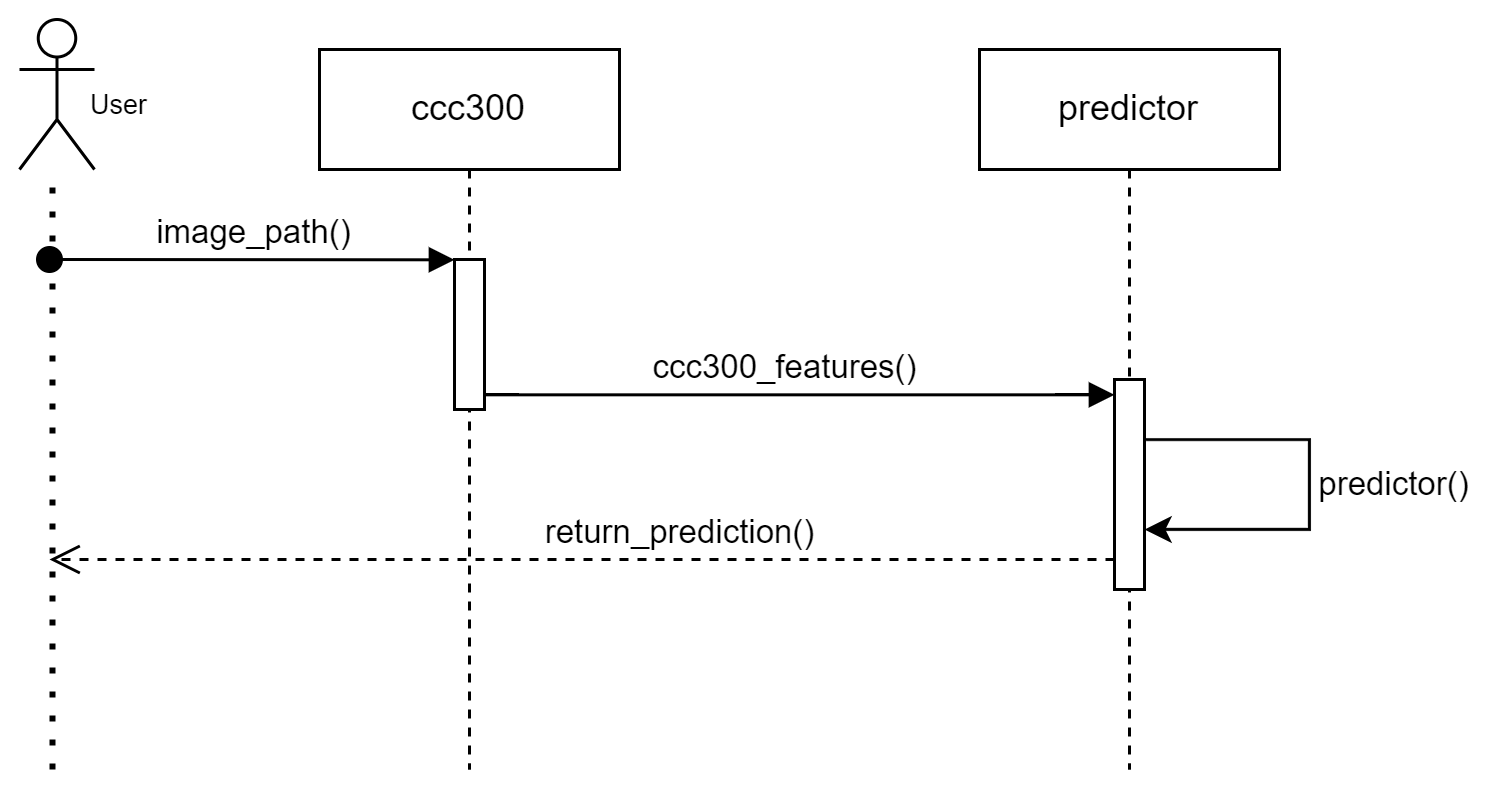
\includegraphics[width=120mm]{./img/sequenceDiagram.png}
    \caption{Sequence Diagram}
\end{figure}
\large{\textbf{Objects}}
\begin{enumerate}[noitemsep]
    \item User
    \item CC-C300
    \item Predictor
\end{enumerate}
\large{\textbf{Steps}}
\begin{enumerate}[noitemsep]
    \item The User sends a message to the CC-C300 extractor to provide the path to the image.
    \item The CC-C300 processes the image, extracts the features and sends a message ``ccc300\_features'' to the Predictor to provide the features.
    \item Finally, the Predictor sends the prediction result back to the User through the message ``return\_prediction()''
\end{enumerate}

\section{SYSTEM BLOCK DIAGRAM}
\begin{figure}[H]
    \centering
    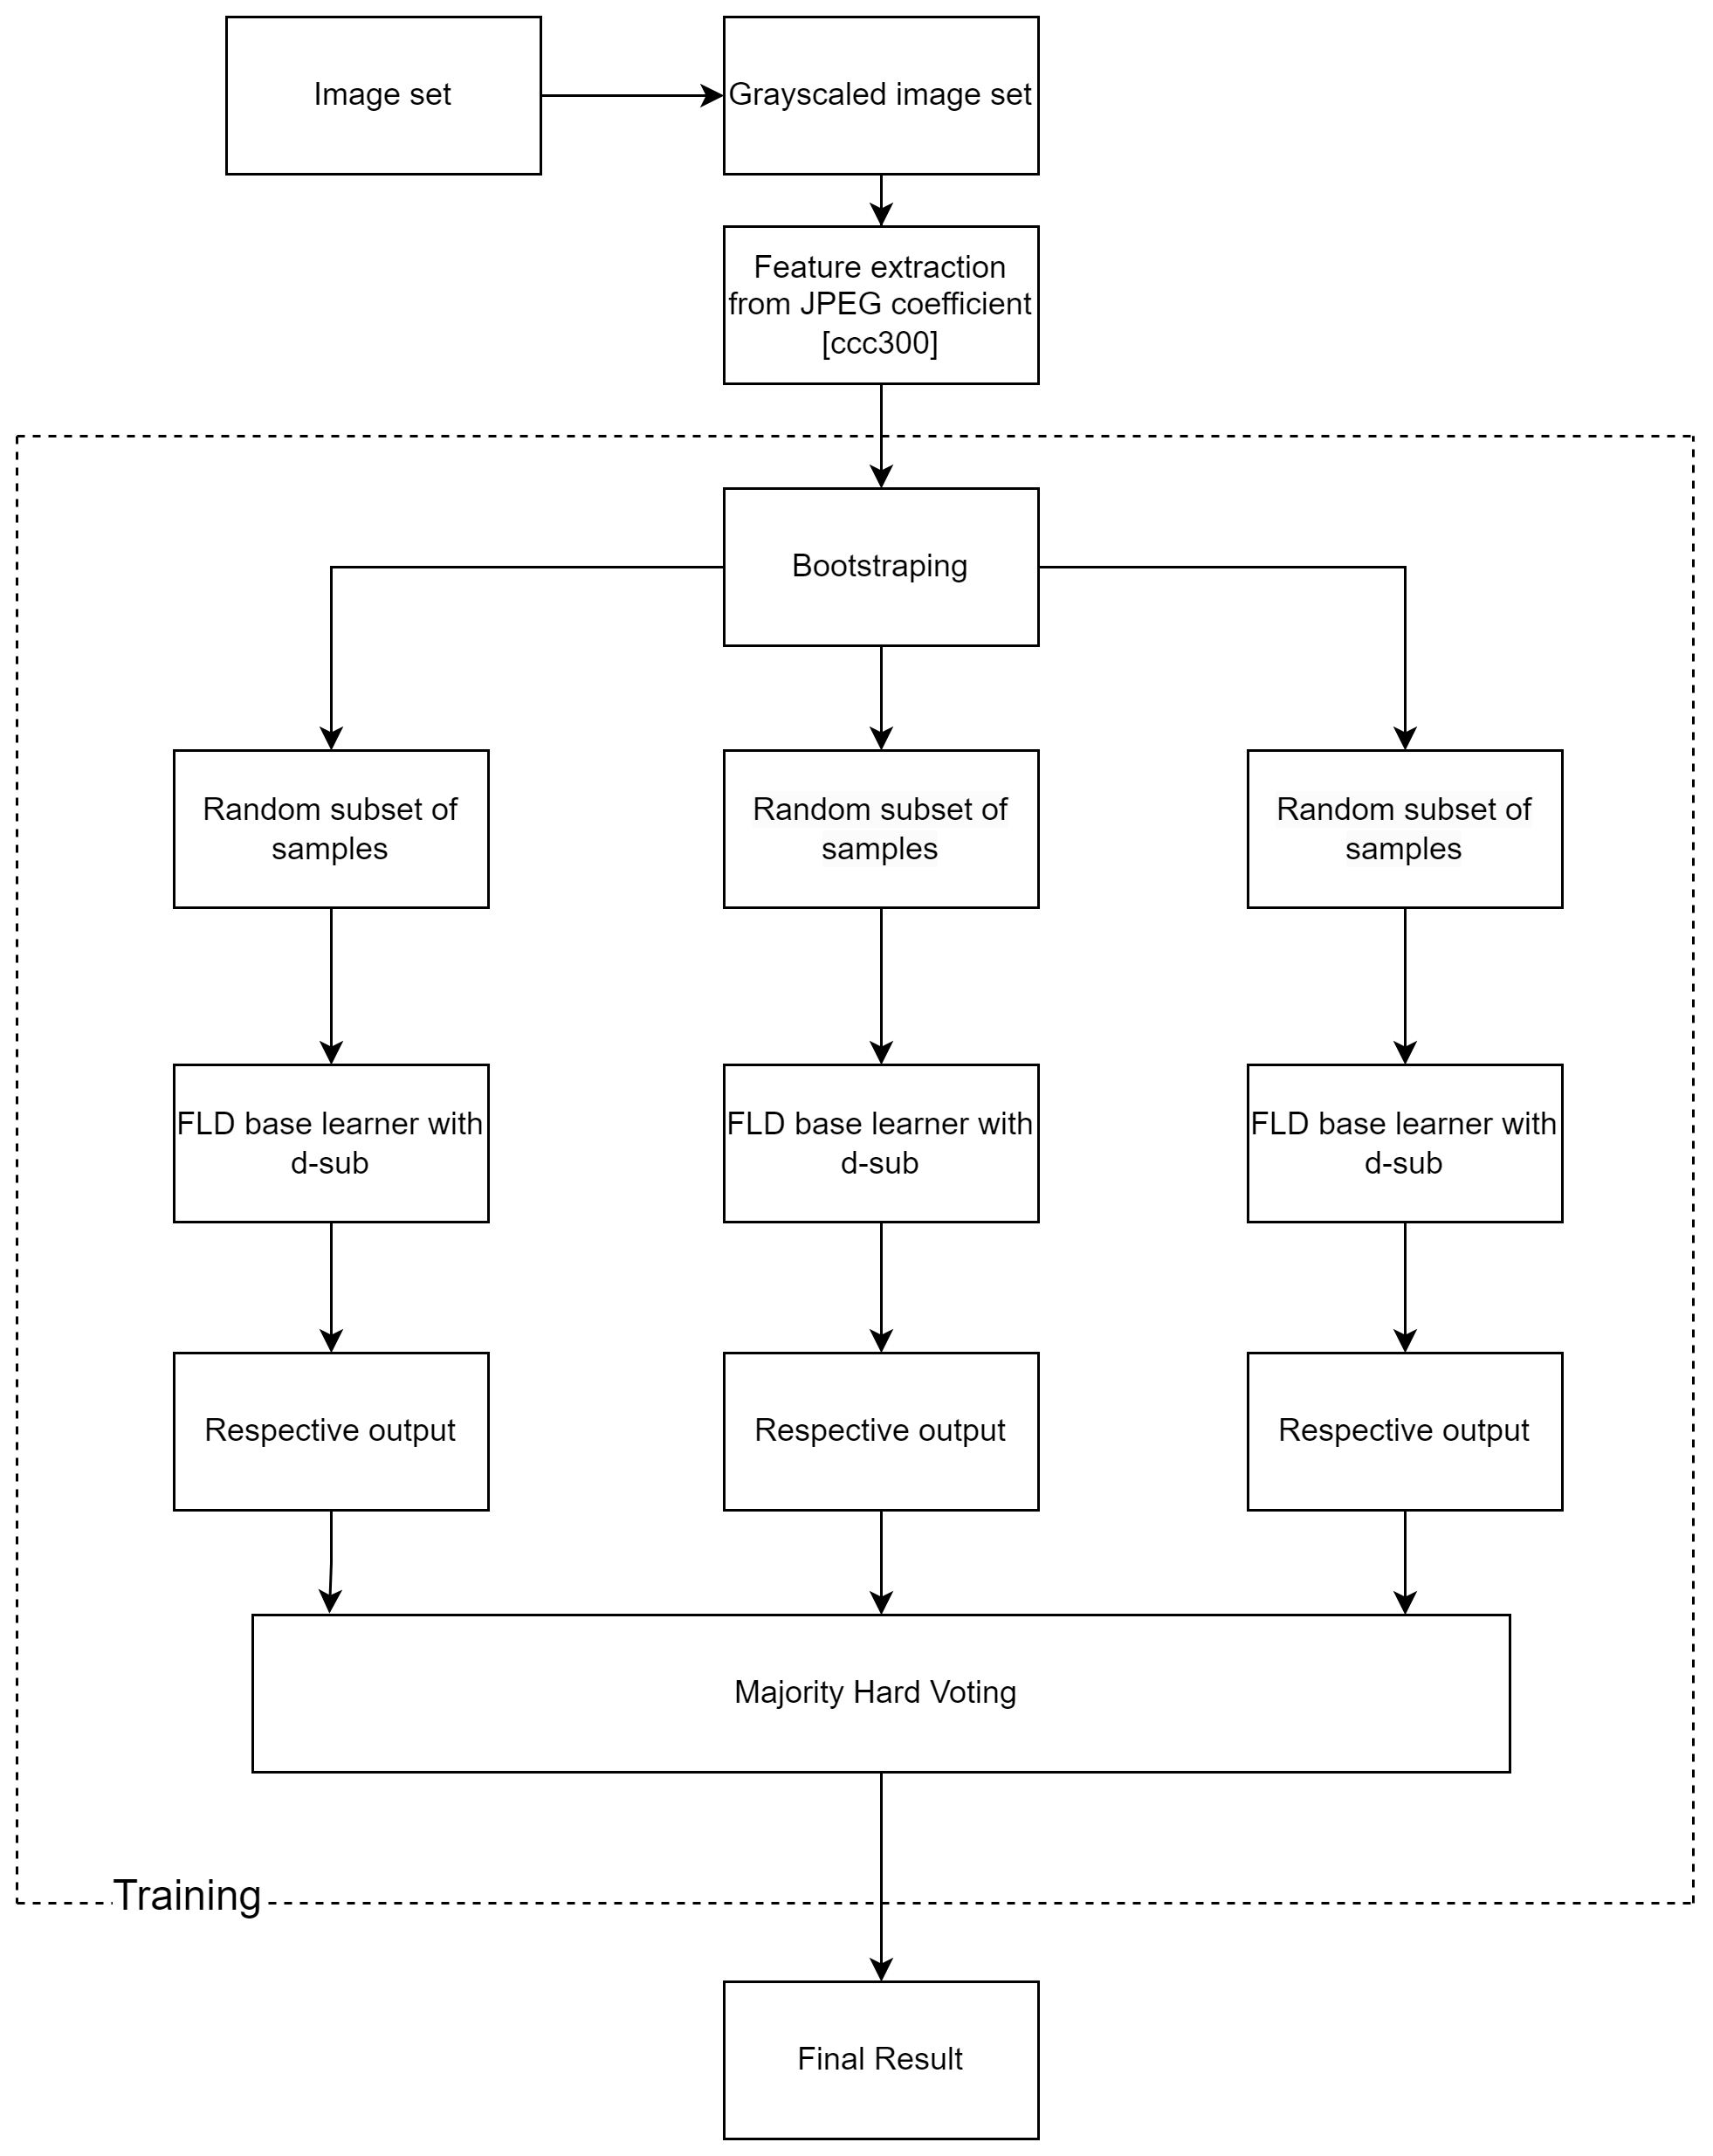
\includegraphics[width=160mm]{./img/blockDiagram.png}
    \caption{System Block Diagram}
\end{figure}
\section{System Architecture}
\begin{figure}[H]
    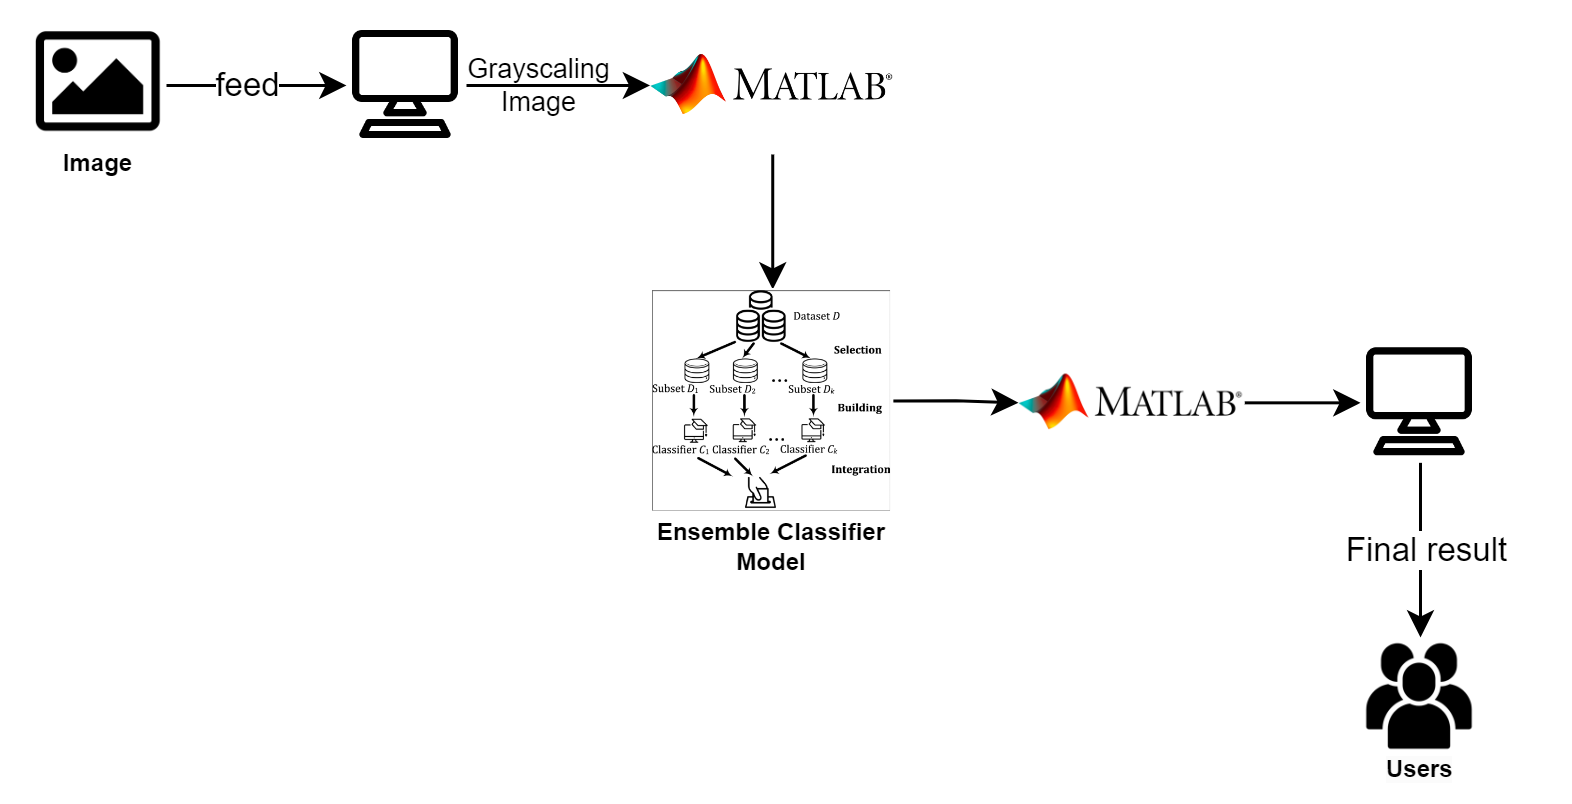
\includegraphics[width=160mm]{./img/architecture.png}
    \caption{System Architecture}
\end{figure}